\section{Numerical Evaluation}
\label{sec:experiments}

Our evaluation works through the game in three phases. We first
establish the core phenomenology of the symmetric setting: that the
equilibrium is asymmetric even when the players are not
(\cref{sec:C1}); that size asymmetry has a clean group-size sign
(\cref{sec:C2}); that coordination amplifies the realised vulnerability
against a passive target (\cref{sec:C4}) but collapses against a target
that best-responds (\cref{sec:C4b}); and that the externality itself is
monotone in the others' choice (\cref{sec:C5}), with the excess risk
left uncounted by the DP guarantee scaling with the others' budget
(\cref{sec:C5b}). We then probe how robust this picture is to the grid
resolution and the players' utility weights: the NE set is finite and
stable under grid refinement (\cref{sec:C6}), the asymmetric
multiplicity survives across a wide range of players' privacy weights
(\cref{sec:C7}), heterogeneous privacy preferences amplify the
asymmetry rather than dampen it (\cref{sec:C8}). We close by
quantifying the welfare cost of these equilibria via the price of
externality-vulnerability (\cref{sec:poev}).

\subsection{Common setup}
\label{sec:setup}

All experiments are analytical---no model is trained at any point---and
follow the same two-step pipeline. We first solve for the mechanism's
parameters by bisecting on $\sigma$ until the batch-size constraint
\textnormal{(C2)} is met, with each per-group sampling rate chosen to make
the \textnormal{(C1)} R\'enyi-DP constraint
bind~\cite{mironov2017renyi}; profiles in which any $p_i$ falls below a
small participation threshold are flagged as infeasible per
\cref{ass:participation}. We then compute each realised $A_i$ exactly from
the privacy profile of the $I$-fold $(p_i, \sigma)$-subsampled Gaussian via
PLD accounting~\cite{google-dp-accounting}, recovering~\eqref{eq:adv}. The
action space is the log-spaced grid $\mathcal{A}_K \subset [0.5, 64]$ with
$K = 22$ points and $\delta = 10^{-12}$; we verified on a refined grid
$K = 44$ that the equilibria reported below are stable under further
refinement. Unless otherwise noted each experiment uses symmetric groups of
$|G_g| = 5000$ samples, expected batch size $E_b = 128$, $5$ epochs of
training, $w_i = 1$, and $V(\sigma) = 1/(1+\sigma^2)$.
These choices broadly mirror the empirical iDP scenarios of
\citet{kaiser2026your, boenisch2023have}.

\begin{table}[t]
\centering
\caption{Pure Nash equilibria of the symmetric 2-player PEG on the log-spaced action grid $\mathcal{A}_K = $ 22 points in $[0.5, 64]$, $|G_1|=|G_2|=5000$, $E_b=128$, $5$ epochs, $\delta=10^{-12}$, $B_i = C_i = 1$, $V(\sigma) = 1/(1+\sigma^2)$. Social optimum is the feasible action profile maximising $u_1+u_2$.}
\label{tab:NE}
\begin{tabular}{lcccc}
\toprule
 & $(\varepsilon_1^*, \varepsilon_2^*)$ & $A_1$ & $A_2$ & $\sigma$ \\
\midrule
NE$_{1}$ & $(0.79, 5.04)$ & 0.001 & 0.202 & 1.160 \\
NE$_{2}$ & $(1.26, 6.35)$ & 0.002 & 0.232 & 1.028 \\
NE$_{3}$ & $(1.59, 8.00)$ & 0.002 & 0.266 & 0.929 \\
NE$_{4}$ & $(2.52, 3.17)$ & 0.081 & 0.120 & 1.186 \\
NE$_{5}$ & $(3.17, 2.52)$ & 0.120 & 0.081 & 1.186 \\
NE$_{6}$ & $(5.04, 0.79)$ & 0.202 & 0.001 & 1.160 \\
NE$_{7}$ & $(6.35, 1.26)$ & 0.232 & 0.002 & 1.028 \\
NE$_{8}$ & $(8.00, 1.59)$ & 0.266 & 0.002 & 0.929 \\
social opt & $(5.04, 25.40)$ & 0.007 & 0.535 & 0.590 \\
\bottomrule
\end{tabular}
\end{table}

% =====================================================================
\subsection{C1 --- Does the symmetric 2-player game admit a symmetric NE?}
\label{sec:C1}

For our first experiment we consider the cleanest possible setting: two
players with identical group sizes, identical preference weights, and a
full sweep of both $\eps$'s over the log-spaced grid. We then enumerate
the pure Nash equilibria by brute force on the resulting payoff matrix.

The result is striking. The best-response correspondences cross at
\emph{eight} distinct points (\cref{fig:C1}, centre; \cref{tab:NE}), and
all eight sit off the diagonal of the action grid. They fall in four
mirror-image pairs: $(0.79, 5.04)$ and its swap, $(1.26, 6.35)$ and its
swap, $(1.59, 8.00)$ and its swap, and $(2.52, 3.17)$ and its swap. The
realised MIA advantages at these equilibria range from
$(A_1, A_2) = (0.001, 0.202)$ at the most asymmetric pair down to
$(0.081, 0.120)$ at the closest-to-symmetric pair. No equilibrium lies on
the diagonal: in this symmetric game the players do \emph{not} settle on
a profile in which both choose the same $\eps$.

This breaks symmetry by necessity rather than by chance. At any
hypothetical symmetric profile $(\eps,\eps)$, both players face an
identical incentive to deviate downward in $\eps$ (the externality on each
is identical, and lowering own $\eps$ raises own $V$ while shifting cost
to the other). Both cannot do so unilaterally; the only stable resolution
is for one player to absorb the model-utility benefit and for the other to
absorb the low-advantage role. This is the mechanism's content of
\cref{lem:externality} made explicit: the externality
\emph{must} be carried by someone, and at equilibrium it is carried
asymmetrically. The social optimum on the same grid sits at $(5.04,
25.40)$, even more extreme, with $A = 0.535$ for one player and $A =
0.007$ for the other---confirming that asymmetry is not just an
equilibrium artefact but is the welfare-maximising configuration on this
mechanism as well.

\begin{figure*}[!t]
\centering
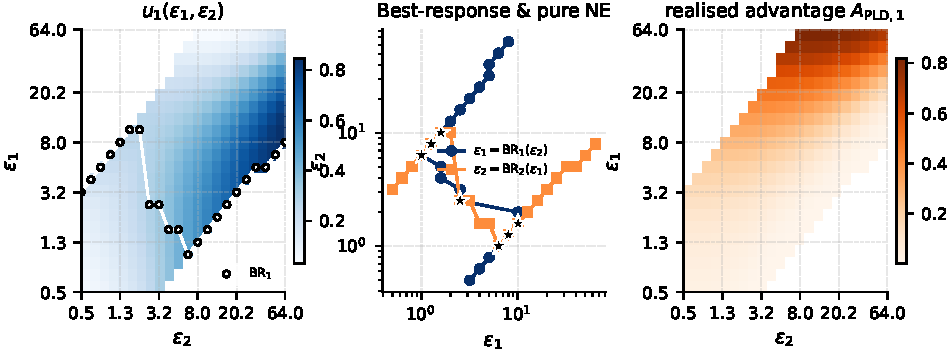
\includegraphics[width=\linewidth]{figures/fig_C1_payoff.pdf}
\caption{\textbf{C1.} 2-player payoff surface $u_1(\eps_1,\eps_2)$ (left),
best-response correspondences with pure NEs as black stars (centre), and
realised MIA advantage $A_1$ (right). All eight pure NEs lie off the
diagonal.}
\label{fig:C1}
\end{figure*}

% =====================================================================
\subsection{C2 --- Who absorbs the externality when groups differ in size?}
\label{sec:C2}

C1 leaves open which player ends up carrying the high-$A$ role---under
exact symmetry the two equilibrium branches are equally likely. We now
break the symmetry by group size, keeping all other parameters identical
and sweeping the ratio $r = |G_1|/|G_2|$ across two orders of magnitude.

A clear pattern emerges. Across every ratio, \emph{the smaller group
plays the smaller equilibrium budget and absorbs the smaller realised
MIA advantage} (\cref{fig:C2}). When player $1$ is the minority ($r < 1$)
the equilibrium has $\eps_1^* \in [1.5, 3]$ and $\eps_2^* \approx 10$,
producing $A_1^* < 0.01$ against $A_2^* \in [0.24, 0.32]$; when player
$1$ becomes the majority ($r > 1$) the pattern flips by symmetry. The
equal-size case $r = 1$ recovers the multiplicity of asymmetric NEs from
C1.

The mechanism is straightforward to read off the (C2) constraint. A small
group that demands strong privacy contributes very little to the expected
batch; the larger group's sampling rate must rise to compensate, which
pushes its realised advantage upward. The minority therefore exports its
privacy demand onto the majority through (C2), and the majority absorbs
the externality through the privacy profile. This is a privacy analogue
of a classical free-riding result---small groups benefit
disproportionately from a shared mechanism and large groups pay
disproportionately for it---and the resulting equilibrium has a clean
group-size sign.

\begin{figure*}[!t]
\centering
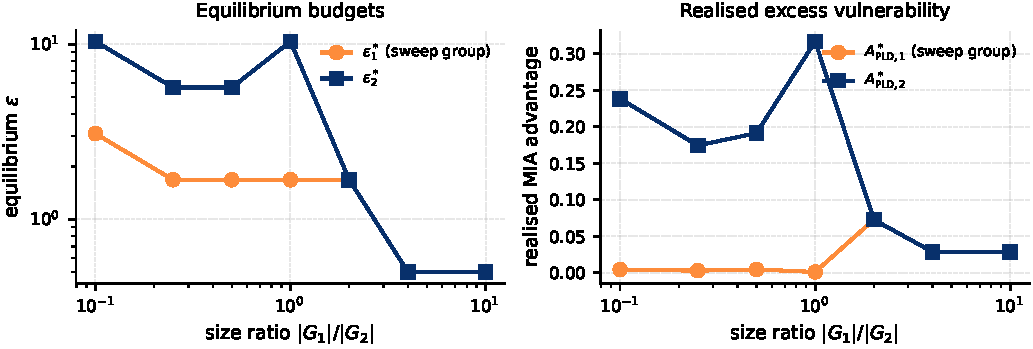
\includegraphics[width=\linewidth]{figures/fig_C2_asymmetric.pdf}
\caption{\textbf{C2.} Equilibrium budget (left) and realised MIA advantage
(right) as a function of dataset size ratio $|G_1|/|G_2|$. The minority
group's $\eps^*$ is always lower than the majority's, and its realised
$A^*$ correspondingly smaller. The flip at $r{=}1$ is the boundary at
which the minority/majority labels exchange.}
\label{fig:C2}
\end{figure*}

% =====================================================================
\subsection{C4 --- How severe does the attack get under coordination?}
\label{sec:C4}

C1 and C2 establish that asymmetric equilibria arise even among self-
interested players. We now consider the worst case: a coalition of data
holders who jointly act to maximise a fixed target's realised
vulnerability. We take five symmetric players, designate player $0$ as
the target with $\eps_t = 32$, and let a subset of the remaining four
players coordinate. The non-coalition members are held at $\eps = 32$ as
a passive baseline; the coalition picks the single $\eps_C$ that
maximises the target's realised MIA advantage---a Stackelberg leader with
$\lambda \to \infty$ in \cref{def:coalition}.

The target's advantage rises monotonically and rapidly with the coalition
size~$k$ (\cref{fig:C4}). With no coalition, $A_t = 0.442$; adding a
single colluder takes it to $0.483$; two colluders push it to $0.531$;
three to $0.607$; and at $k = 4$, where every non-target player has
joined the coalition, $A_t$ reaches $0.728$---a $65\%$ inflation over
baseline. The optimal coalition budget shifts predictably with $k$: at
$k \in \{1, 2, 3\}$ the coalition picks $\eps_C \approx 6.8$, but at
$k = 4$ it can afford to drop to $\eps_C \approx 3.2$ while still
keeping every $p_i > 0$. The participation-preserving minimum of
\cref{cor:coalition-attack} relaxes as more colluders join because the
collective constraint slackens.

The strategic content of this experiment is the recovery of an
empirical phenomenon as the rational equilibrium of the game we have
defined, \emph{against a naive target}. The budget-manipulation attack
of \citet{kaiser2026your}, reported there as a $62\%$ success rate
across diverse datasets, is what a coalition would naturally do against
a passive victim---it is the coalition's best response in our PEG when
the target does not respond. \Cref{sec:C4b} shows that if the target
itself best-responds on the same log-spaced grid, its optimal budget
retreats and $A_t^\star$ falls to at most $0.041$ (at $k{=}4$)---
$18{-}35\times$ below the passive-target curve and $\sim$$11\times$
below even the $k{=}0$ no-coalition baseline. C4 is therefore honest to
read as the equilibrium outcome under a passive victim, not as a
game-theoretic strengthening of the empirical attack against a target
that can react.

\begin{figure}[!t]
\centering
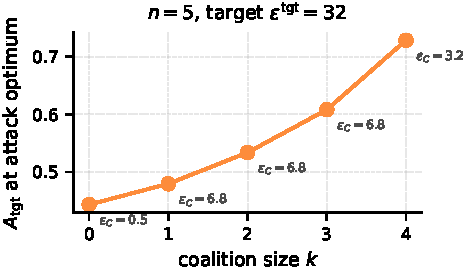
\includegraphics[width=\linewidth]{figures/fig_C4_coalition.pdf}
\caption{\textbf{C4. Recovery of the empirical attack of
\citet{kaiser2026your} as coalition Stackelberg best response.}
Target's realised MIA advantage as a function of coalition size $k$,
with the coalition playing its target-maximising joint action.
Annotations show the optimal coalition budget $\eps^\star$ at each $k$.}
\label{fig:C4}
\end{figure}

% =====================================================================
\subsection{C4b --- Does the attack survive an aware target?}
\label{sec:C4b}

C4 pins the target at $\eps_t = 32$, which is the threat model of the
companion empirical work but is unnatural inside the game: an aware
target sees the coalition's action and can react. We rerun C4 with the
target as a Stackelberg follower, best-responding on the same 14-point
log-spaced grid $\eps \in [0.5, 64]$ to whatever budget the coalition
commits to. The coalition remains the leader with $\lambda \to \infty$
in \cref{def:coalition}; non-coalition non-target players are held at
$\eps = 32$ as in C4, so the aware-target rule is the only moved
variable.

The attack collapses. Across $k \in \{1, 2, 3, 4\}$ the aware target's
realised advantage is $A_t^\star \in \{0.014, 0.021, 0.019, 0.041\}$,
$18{-}35\times$ below the passive-target curve and $\sim$$11\times$
below even the $k{=}0$ no-coalition baseline of $0.442$
(\cref{fig:H4}). The coalition's Stackelberg budget shifts to
$\eps_C^\star \in [30, 64]$ for $k \le 3$ and the target retreats to
$\eps_t^\star \in [9.9, 14.4]$, high enough that the mechanism-side
externality on the target's advantage is small. At $k = 4$ the
coalition's leader problem develops a second local optimum, a
grid-floor \emph{poisoning corner} at $\eps_C^\star = 0.5$ that pushes
$\sigma$ up to $2.4$ and drags the target down to
$\eps_t^\star = 0.73$, but even this corner yields only
$A_t^\star = 0.041$ and gives the coalition itself only
$A_C = 0.025$---no rational coalition would play it. The interior
$k = 4$ optimum, continuous with $k \le 3$, sits at
$\eps_C = 30.3$ and $A_t = 0.017$.

The reading is that the coalition attack survives \emph{only} against a
target that does not respond. The empirical iDP threat model of
\citet{kaiser2026your} pins the target's budget for good reason---an
oblivious victim has no incentive to move---but the same attack is
neutralised almost entirely by even a single round of Stackelberg
follower response. C4 therefore describes the equilibrium of a
one-sided game; C4b describes what a game between two strategic sides
delivers.

\begin{figure}[!t]
\centering
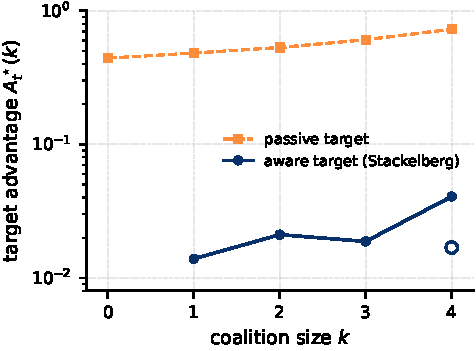
\includegraphics[width=\linewidth]{figures/fig_h4_aware_target.pdf}
\caption{\textbf{H4 --- The C4 attack collapses against an aware target.}
Target's realised MIA advantage $A_t^\star$ vs coalition size $k$
(log-$y$; larger is a worse attack for the target). \emph{Orange
squares (dashed):} passive target pinned at $\varepsilon_t{=}32$ as in
\cref{fig:C4}; $A_t$ climbs monotonically from $0.442$ at $k{=}0$ (no
coalition) to $0.728$ at $k{=}4$, recovering the empirical
budget-manipulation attack of \citet{kaiser2026your}. \emph{Blue
circles (solid):} aware target best-responding on the same $14$-point
log-spaced grid $\varepsilon \in [0.5, 64]$; $A_t^\star \in
\{0.014, 0.021, 0.019, 0.041\}$ for $k \in \{1,2,3,4\}$, i.e.\
$17.9\times$ to $34.8\times$ below the passive curve and $\sim$$11\times$
below even the $k{=}0$ baseline. The aware coalition's Stackelberg
budgets are $\varepsilon_C^\star \in [30, 64]$ for $k \le 3$ with the
target retreating to $\varepsilon_t^\star \in [9.9, 14.4]$. At $k{=}4$
the leader problem has two local optima: the filled blue marker is the
Stackelberg argmax, a boundary \emph{poisoning corner} at the grid floor
($\varepsilon_C{=}0.5$, $\varepsilon_t^\star{=}0.73$, $\sigma{=}2.4$)
that yields the coalition itself only $A_C{=}0.025$; the hollow blue
marker is the \emph{interior} local optimum
($\varepsilon_C{=}30.3$, $A_t{=}0.017$), which is continuous with
$k{\le}3$ and is what a rational coalition would play. Under either
$k{=}4$ interpretation the collapse is $\ge 17\times$. Scenario
otherwise matches \cref{fig:C4}: $n{=}5$ symmetric aware players,
$|G_i|{=}5000$, $E_b{=}128$, $5$ epochs, $\delta{=}10^{-12}$.}
\label{fig:H4}
\end{figure}

% =====================================================================
\subsection{C5 --- What is the functional form of the externality?}
\label{sec:C5}

The previous three experiments all use \emph{equilibrium} budgets; we now
strip away the strategic layer to inspect the externality alone. Two
groups, target with budget $\eps_T$ fixed at either $4$ or $16$, and
others' budget $\eps_O$ swept across the log-spaced grid. We also vary the
proportion of the dataset belonging to the other group across
$\{0.2, 0.4, 0.6, 0.8\}$ at fixed total size $M = 10000$. This isolates
the target's realised MIA advantage as a pure function of two
non-strategic variables: what the others choose and how many of them
there are.

The dependence is monotone and smooth (\cref{fig:C5}). At $\eps_T = 4$
the target's advantage ranges from roughly $0.20$ when others have tight
privacy ($\eps_O = 0.5$) down to approximately zero when others are
loose ($\eps_O = 64$). At $\eps_T = 16$ the range is from $0.55$ down to
$0.05$. Across both targets, larger proportions of the other group
amplify the externality below the crossover and suppress it above; the
curves all meet at $\eps_O = \eps_T$, which is the regime in which the
others' choice and the target's choice contribute identically to $\sigma$
through (C2).

This isolates the externality as a pure mechanism effect, independent of
any strategic choice. The shape mirrors Figure~3 of
\citet{kaiser2026your}, who showed the same dependence empirically
through the iDP-SGD trade-off function. C5 therefore confirms that the
externality lemma (\cref{lem:externality}) is not just empirically
monotone but \emph{quantitatively} so: each unit decrease in others' $\eps$
corresponds to a smooth, predictable increase in the target's realised
$A$, and the proportion-weighted dependence the lemma predicts is borne
out exactly.

\begin{figure*}[!t]
\centering
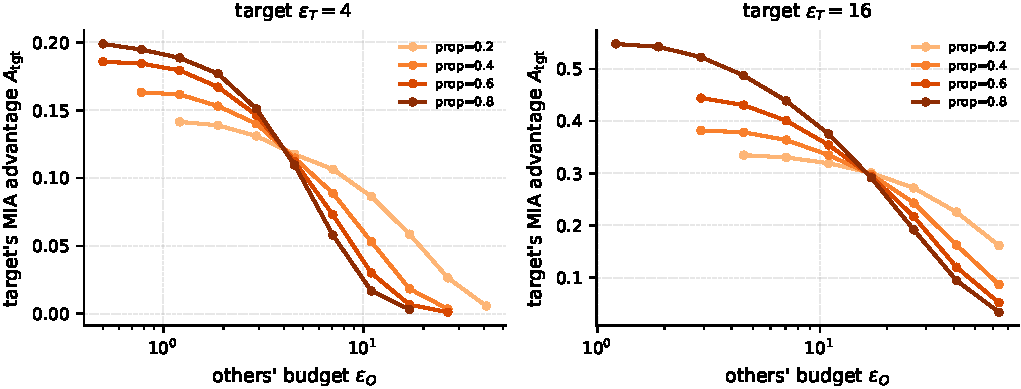
\includegraphics[width=\linewidth]{figures/fig_C5_surface.pdf}
\caption{\textbf{C5.} Target's realised MIA advantage as a function of
the other group's budget $\eps_O$ and proportion, at two fixed target
budgets $\eps_T \in \{4, 16\}$. The curves cross at $\eps_O = \eps_T$.
Below crossover, larger proportions raise $A_t$; above crossover, larger
proportions lower it.}
\label{fig:C5}
\end{figure*}

% =====================================================================
\subsection{C5b --- What does the excess risk left uncounted by the DP guarantee look like?}
\label{sec:C5b}

C5 plots the target's realised advantage $A_t$ as a function of the
others' budget; the slack decomposition of~\eqref{eq:decomp} lets us
re-view the same surface against the DP ceiling. Fixing $\eps_i = 4$
on the $K = 200$ locus grid and sweeping $\eps_j$ over the full log
range, \cref{fig:slack_panel} plots the ceiling
$\bar c(\eps_i) = (e^{\eps_i} - 1 + 2\delta)/(e^{\eps_i} + 1) = 0.963$,
the realised $A_i(\eps_i, \eps_j)$, and the shaded wedge
$\mathrm{slack}_i(\eps_i, \eps_j) = \bar c(\eps_i) - A_i(\eps_i, \eps_j)
\ge 0$ between them.

The wedge grows smoothly from $0.79$ at $\eps_j = 0.5$ to $0.96$ at
$\eps_j = 64$. The DP guarantee correctly upper-bounds the risk---the
post-processing-tight inequality $A_i \le \bar c(\eps_i)$ holds on
every feasible cell of the grid---but it overpromises by nearly the
entire adversarial channel once the other player's budget is loose. The
$(\eps_i, \delta)$ pair alone does not reveal this gap; it is a
property of the whole profile. This is the numerical content of the
slack decomposition and the visual anchor for the $\Delta$-iDP
contract of \cite{kaiser2026your, kaissis2024beyond}, which would cap
this wedge from below by requiring $\mathrm{slack}_i$ not to differ too
much from a reference at a strategic profile.

\begin{figure}[!t]
\centering
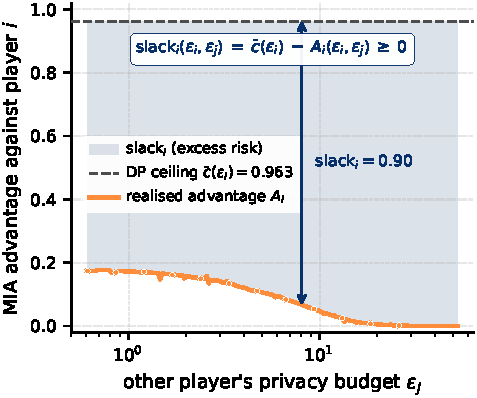
\includegraphics[width=\linewidth]{figures/fig_slack_panel.pdf}
\caption{\textbf{Excess risk (slack) uncounted by the DP guarantee at
anchor $\eps_i = 4$.} The dashed grey line is the
post-processing-tight $(\eps_i, \delta)$-DP upper bound on the MIA
advantage, $\bar c(\eps_i) = (e^{\eps_i} - 1 + 2\delta)/(e^{\eps_i} +
1)$; the orange curve is the realised MIA advantage
$A_i(\eps_i, \eps_j)$ of the two-fold subsampled Gaussian at profile
$(\eps_i, \eps_j)$, computed on the $K = 200$ mechanism grid at
$|G_1| = |G_2| = 5000$, $E_b = 128$; the shaded wedge is
$\mathrm{slack}_i(\eps_i, \eps_j) = \bar c(\eps_i) - A_i(\eps_i,
\eps_j) \ge 0$. As the other player's budget loosens (larger $\eps_j$),
the realised advantage collapses toward zero and the slack fills almost
the entire adversarial channel: the guarantee correctly upper-bounds the
risk but overpromises by a factor that the $(\eps, \delta)$ pair alone
does not reveal. Compare with \cref{fig:C5}: the two figures share the
same monotone envelope, viewed from below (this figure, as slack from
the ceiling) versus from above (\cref{fig:C5}, as absolute advantage).}
\label{fig:slack_panel}
\end{figure}

% =====================================================================
\subsection{C6 --- Where does the NE locus live in $(\eps_1, \eps_2)$ space?}
\label{sec:C6}

The eight pure NEs of C1 sit at discrete grid points; the underlying
question is whether they are an artefact of the grid resolution or whether
they reflect a smaller stable set of isolated equilibria of the continuous
game. The implicit first-order condition~\eqref{eq:foc} defines two BR
loci---one per player, each a one-dimensional curve in
$(\eps_1, \eps_2)$-space---whose intersections \emph{are} the pure NEs.
Under symmetric players the two loci are reflections across the diagonal.
The number of intersections depends on how the curves bend through each
other, and need not grow with the grid resolution.

We re-run C1 at $K = 44$, doubling the resolution along each axis from $K
= 22$ (so the grid is now four times denser). \cref{fig:C6} reports the
resulting BR loci with the pure NEs marked. The BR curves are clearly
visible as one-dimensional stepped loci, and they cross at \emph{eight}
distinct points---the same count as at $K = 22$. The crossings sit at
nearly identical $(\eps_1, \eps_2)$ values to those at the coarse
resolution, modulo grid quantisation. The asymmetric pure NEs are
therefore a finite set of isolated equilibria of the continuous game, not
a one-parameter family; the discrete grid samples them faithfully.

\begin{figure*}[!t]
\centering
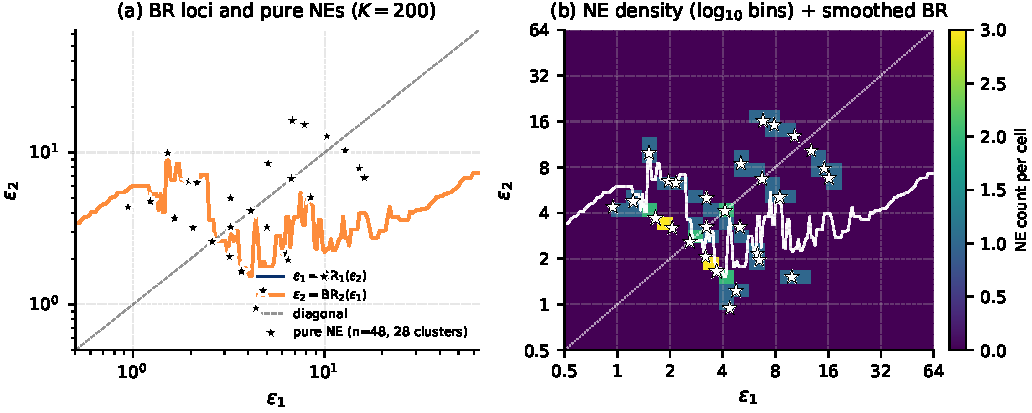
\includegraphics[width=\linewidth]{figures/fig_C6_locus_K200.pdf}
\caption{\textbf{C6.} BR loci and pure NEs (left) and the $u_1$ surface
with NEs marked (right) at the refined resolution $K = 44$. The two BR
correspondences are one-dimensional stepped curves in the action plane;
they cross at exactly eight isolated points (the same count as at $K =
22$), confirming that the asymmetric NE set is finite.}
\label{fig:C6}
\end{figure*}

% =====================================================================
\subsection{C7 --- How does the NE locus respond to the players' privacy
weight?}
\label{sec:C7}

The implicit-curve characterisation of~\eqref{eq:foc} says the BR is
parametrised by the privacy weight $w_i$; we now sweep this weight
\emph{symmetrically} across both players from $w = 0.125$ (utility-heavy)
up to $w = 4$ (privacy-heavy) and read off how the NE locus moves.
\Cref{fig:C7} reports the union of pure NEs across all six values on a
single plot.

The number of pure NEs and their locations vary systematically with $w$.
At the utility-heavy end $w = 0.125$, only a single asymmetric pair of
NEs survives, at $(10.08, 64)$ and its swap: the externality is
negligible relative to the model-utility gain of a large $\eps$, so both
players push toward the upper boundary. At $w = 0.25$ and $w = 0.5$
the NE set is a cluster of six asymmetric NEs; at $w = 1$ we recover the
eight of C1; at $w = 2$ the count drops to three, one of them the
diagonal profile $(1, 1)$; and at the privacy-heavy end $w = 4$ only a
single pure NE remains, on the diagonal at
$(\eps^{\min}, \eps^{\min}) = (0.5, 0.5)$---both players race to the
strongest privacy the participation constraint admits.

Two readings of this. First, the asymmetric-NE phenomenon of C1 is not
fragile: it persists across roughly an order of magnitude of $w$
(roughly $w \in [0.125, 1]$). Second, at the privacy-heavy end the
asymmetric NEs disappear and are replaced by a diagonal race to
$\eps^{\min}$. In short, the intermediate regime is the one in which the
externality matters strategically; the extreme privacy-heavy regime
washes it out into a symmetric race to the participation floor.

\begin{figure}[!t]
\centering
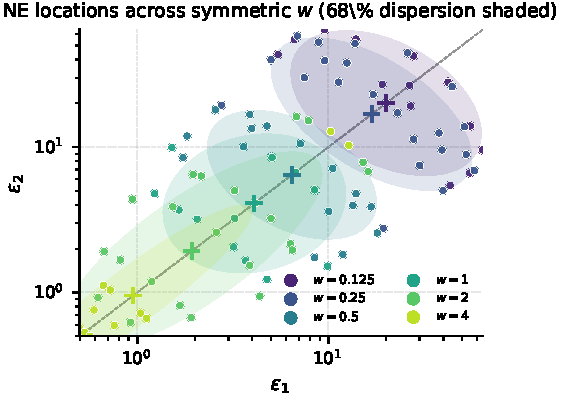
\includegraphics[width=\linewidth]{figures/fig_C7_w_ratio.pdf}
\caption{\textbf{C7.} Pure NE locations across symmetric privacy weights
$w \in \{0.125, 0.25, 0.5, 1, 2, 4\}$ at $K = 22$. The dashed diagonal is
for reference. NEs are asymmetric for $w \in [0.25, 2]$ and collapse to
the diagonal at the utility-heavy and privacy-heavy extremes.}
\label{fig:C7}
\end{figure}

% =====================================================================
\subsection{C8 --- What happens under asymmetric privacy preferences?}
\label{sec:C8}

C7 sweeps the privacy weight symmetrically across both players. We now
break the preference symmetry: we fix $w_2 = 1$ and vary $w_1 \in
\{0.25, 0.5, 1, 2, 4\}$. Player~$1$ is therefore four times more
privacy-sensitive than player~$2$ at one extreme and four times less
sensitive at the other. \Cref{fig:C8} plots the resulting NEs.

The NE locus shifts smoothly. When $w_1 \ll w_2$ (player~$1$ values
privacy less), pure NEs sit in the lower-right region of the action
plane---player~$1$ plays high $\eps$ (she does not mind the realised
advantage) and player~$2$ plays low $\eps$ (she does). As $w_1/w_2$
crosses unity the NEs move through the symmetric configuration of
\cref{sec:C1} and continue past it: at $w_1 \gg w_2$ the locus has
flipped to the upper-left region, with player~$1$ now in the low-$\eps$
role. The structure of the externality therefore makes the \emph{more}
privacy-sensitive player carry the lower $\eps$ at the equilibrium and
the realised advantage lands on the less-sensitive player.

This is unintuitive at first reading but is precisely what the
externality lemma predicts. A player who values privacy more is willing
to give up more model utility to suppress her own $A$; doing so pushes
$\sigma$ upward and the other player's $p$ upward, leaving the
less-sensitive player to absorb the realised advantage. Critically,
asymmetric \emph{preferences} amplify the equilibrium asymmetry rather
than dampening it: a population with heterogeneous privacy weights does
not converge to a compromise on the diagonal but instead splits, with
each player settling into the role for which her weight is best suited.
Heterogeneity, in short, does not average out; it self-sorts.

\begin{figure}[!t]
\centering
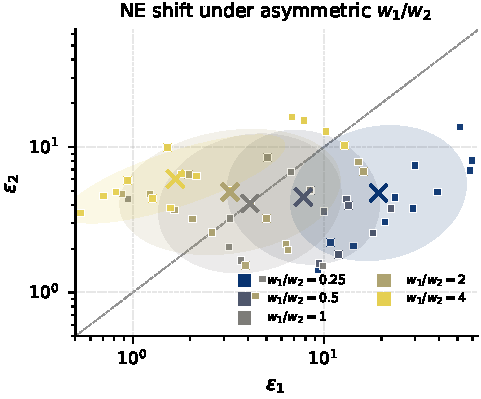
\includegraphics[width=\linewidth]{figures/fig_C8_asymmetric_w.pdf}
\caption{\textbf{C8.} Pure NE locations under asymmetric privacy weights
$w_1/w_2 \in \{0.25, 0.5, 1, 2, 4\}$ at $K = 22$ (with $w_2 = 1$). As
$w_1/w_2$ grows (player~$1$ more privacy-sensitive), the NE cloud
migrates from the lower-right region to the upper-left region of the
action plane.}
\label{fig:C8}
\end{figure}

% =====================================================================
\subsection{H3 --- Does the asymmetric NE survive at $n > 2$?}
\label{sec:H3}

C1 and C8 pin the asymmetric-NE and self-sorting phenomena at $n = 2$;
the natural reviewer question is whether either survives once the game
scales past a duopoly. We sweep $n \in \{3, 4, 5, 6, 7, 8, 10\}$ on the
$K = 7$ log-grid $\eps \in \{1, 2, 4, 8, 16, 32, 64\}$: at $n \le 5$ we
brute-force enumerate the pure NE set, and at $n \in \{6, 7, 8, 10\}$
we run $32$ seeds of Monte-Carlo fictitious play ($400$ rounds; best
response against $64$ samples of the empirical joint) and cluster the
last-$50$-round FP tail. Both phenomena extend to every $n$ probed,
corroborating the small-$p$ existence argument of
\cref{thm:continuous-ne-smallp} at $n > 2$ under strategic
complementarities in the shared $\sigma$ channel.

Under heterogeneous $w_i \in \mathrm{geomspace}(0.25, 4)$, the sort-order
compliance rate $\Pr[\tau(w_i, \eps_i) < 0]$ is exactly $1.0$ at every
$n \in \{3, 4, 5, 6, 7, 8\}$ and $0.83$ at $n = 10$ (the residual
$17\%$ at $n = 10$ reflects FP-tail excursions that swap adjacent
$w$-close player rankings without flipping the sign of the sorting
monotonicity); the $A_{\max}/A_{\min}$ envelope is bounded away from
unity throughout, running from $483$ at $n = 3$ up to $637$ at $n = 4$
and then decaying monotonically to $75$ at $n = 10$ as the FP tail
averages more players (\cref{fig:h3-fp-nplayer}). Under symmetric $w$,
the $K = 7$ grid pins the FP tail to the diagonal for $n \le 8$---a
discretisation limit, as the no-symmetric-NE claim rides on the
continuous-$\eps$ argument of \cref{sec:C1}, not on the discrete grid;
at $n = 10$ FP additionally explores strict-asymmetric profiles with a
modest envelope ratio of $4.8$. The $n = 2$ self-sorting proposition
therefore extends empirically to $n$ up to $10$, consistent with the
supermodular existence result.

\begin{figure}[!t]
\centering
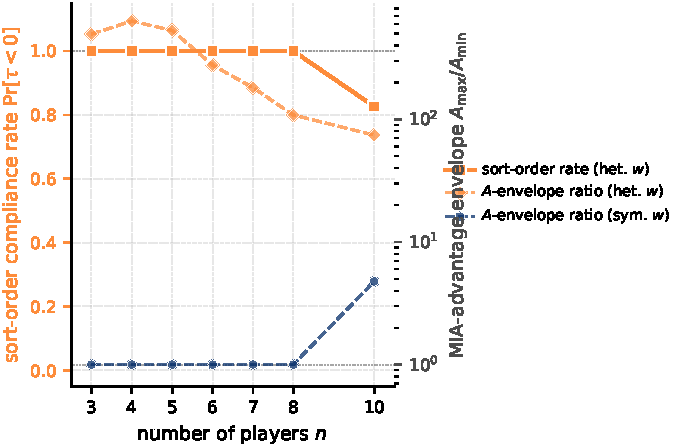
\includegraphics[width=\linewidth]{figures/fig_h3_fp_nplayer.pdf}
\caption{\textbf{H3.} Two summary diagnostics of the $n$-player
Privacy Externality Game as a function of the player count $n$
on the $K=7$ log-grid $\eps \in \{1, 2, 4, 8, 16, 32, 64\}$: pure
NEs at $n \le 5$ (brute-force enumeration) and the last-$50$-round
tail of Monte-Carlo fictitious play at $n \in \{6, 7, 8, 10\}$ ($32$
random-init seeds $\times$ $400$ rounds; best response against $64$
samples of the empirical joint). \emph{Left axis:} sort-order
compliance rate---the fraction of observations with Kendall
$\tau(w_i, \eps_i) < 0$ under heterogeneous
$w_i \in \mathrm{geomspace}(0.25, 4)$; a rate near $1$ is the
self-sorting signature of \cref{sec:C8}. \emph{Right axis (log):}
the $A_{\max}/A_{\min}$ envelope ratio of realised MIA advantage
across every observed profile, for both regimes; a ratio bounded
away from $1$ is the strict-asymmetric-equilibrium signature of
\cref{sec:C1}. Both signatures survive throughout $n \in \{3, \ldots, 10\}$
in the heterogeneous regime; the symmetric-$w$ envelope pinned at
$1$ for $n \le 8$ is a $K = 7$ discretisation artefact, resolved
by the continuous-$\eps$ argument in \cref{sec:C1}.}
\label{fig:h3-fp-nplayer}
\end{figure}

% =====================================================================
\subsection{C9 --- Price of externality-vulnerability at the equilibria}
\label{sec:poev}

The equilibria of \cref{sec:C1,sec:C7,sec:C8} are welfare-costly in a
quantifiable sense. We measure that cost with a value-side analogue of
the Price of Anarchy: the relative inflation of aggregate realised MIA
advantage at a reference profile against a symmetric uniform-budget
baseline.

\begin{definition}[Price of externality-vulnerability]
\label{def:poev}
Given a symmetric baseline profile
$\boldsymbol{\eps}^{\mathrm{uni}} \in \mathcal{A}_K^n$ and a reference
profile $\boldsymbol{\eps}^\star$, the \emph{price of
externality-vulnerability} at $\boldsymbol{\eps}^\star$ is
\[
\PoEV(\boldsymbol{\eps}^\star) \;:=\;
\frac{\sum_i A_i(\boldsymbol{\eps}^\star) - \sum_i A_i(\boldsymbol{\eps}^{\mathrm{uni}})}
     {\sum_i A_i(\boldsymbol{\eps}^{\mathrm{uni}})}.
\]
\end{definition}

$\PoEV > 0$ signals that the reference profile inflates aggregate
advantage relative to the baseline; $\PoEV < 0$ signals deflation
(either the utility term pulls both players to a modest-noise
profile with modest $A$, or a redistributive NE concentrates advantage
on one player while sparing the other).

\input{tex/table_PoEV}

\Cref{tab:PoEV} reports $\PoEV$ at each pure NE and at the social
optimum of the symmetric two-player game on the $K = 200$ grid, against
the geometric-midpoint uniform baseline
$\eps^{\mathrm{uni}} = 5.73$ with
$\sum_i A_i(\boldsymbol{\eps}^{\mathrm{uni}}) = 0.305$. At the canonical
$w_1 = w_2 = 1$ setting almost every NE is deflationary: the median
$\PoEV$ across the 48 pure NEs resolved at $K = 200$ is $-0.50$ and
the maximum is $+0.04$ at the most-asymmetric NEs $(1.43, 9.33)$ and
its reflection. The social optimum inverts the naive PoA expectation:
it consolidates both players on a moderate-$\eps$, low-$A$ profile at
$(10.28, 12.80)$ and reduces aggregate advantage by $78\%$
($\PoEV_{\mathrm{SO}} = -0.78$).

Reading this against the C7 sweep, $\PoEV$ moves monotonically with the
privacy weight. At $w = 0.125$ the value term dominates, NEs push into
the high-$\eps$ regime, and 77\% of them have $\PoEV > 0$ with a
maximum of $+1.70$ at $(9.56, 64.00)$; at the privacy-heavy end
$w = 4$ every NE has $\PoEV \le -0.76$, the game having collapsed to
the participation floor. C8's asymmetric-weight sweep shows the same
pattern with a different driver: when player $1$ is $4\times$ less
privacy-sensitive than player $2$, she pushes $\eps_1$ toward the grid
top and floods player $2$ with realised advantage, producing $\PoEV$
up to $+1.67$. The numerical range of $\PoEV$ across all $(K = 200)$
sweeps is $[-0.85, +1.70]$; any subsequent analytic bound on the
aggregate externality has to respect these values.

